\chapter{Full Wave Rectifier}
\vspace{-1cm}

%--------------------------AIM-----------------------------
\section{Aim}
\hspace{1cm}To design and implement Single Phase Full Wave Uncontrolled and Controlled rectifiers, and
simulate them with R and RL loads.

%--------------------------SOFTWARE USED-----------------------------
\section{Software Used}
\hspace{1cm}MATLAB R2020a
%-------------------------THEORY---------------------------
\section{Theory}
\hspace{\parindent}

A full-wave rectifier is an electronic circuit that converts an alternating current (AC) input signal into a unidirectional pulsating direct current (DC) output signal. It is a rectifier that uses both halves of the input sinusoidal waveform. It is essentially two half-wave rectifiers connected together to feed the load. The rectification is done by passing the positive half of the waveform while inverting the negative half of the sine wave. This results in a pulsating DC output. However, the output does not reverse direction, as it uses the full 100% of the input waveform, resulting in full-wave rectification.

The full-wave rectifier is a more efficient rectifier compared to the half-wave rectifier because it produces a smoother DC output. Additionally, it has a higher output voltage and lower output ripple than a half-wave rectifier.

In a single-phase full-wave rectifier, four diodes are used in a bridge configuration to rectify the AC input signal. The input AC voltage is applied across the two AC input terminals of the rectifier, and the output voltage is taken from the two DC output terminals. The four diodes are connected in such a way that the input voltage is rectified, producing a DC output voltage across the output terminals.

The four diodes used in the bridge rectifier are arranged in a way such that when the AC input voltage is positive, diodes D1 and D3 are forward-biased and conduct, while diodes D2 and D4 are reverse-biased and do not conduct. Conversely, when the AC input voltage is negative, diodes D2 and D4 are forward-biased and conduct, while diodes D1 and D3 are reverse-biased and do not conduct. This process of rectification occurs for each half-cycle of the AC input voltage, producing a unidirectional DC output signal.

% \vspace{1cm}

%----------------------Theoretical Calculations----------------------
\section{Theoretical Calculations}
\hspace{\parindent}
In the theory of full-wave rectifiers, the average output voltage and current for controlled full-wave rectifiers with resistive (R) load can be calculated using the following equations:

\begin{equation}
    V_0 = \frac{V_{phase}}{\sqrt{2}}\frac{(1+\cos\alpha)}{\pi}
\end{equation}

\begin{equation}
    V_0 = \frac{V_m(1+\cos\alpha)}{2\pi}
\end{equation}

\begin{equation}
    I_0 = \frac{V_0}{R}
\end{equation}

where $\alpha$ is the thyristor's firing angle. It should be noted that in uncontrolled rectifiers, the thyristor is switched out for a diode and $\alpha$ is equal to 0.

For a single-phase full-wave uncontrolled rectifier, the average output voltage and current can be calculated as follows:

\begin{equation}
    V_0 = 2\sqrt{2}V_{rms}
\end{equation}

\begin{equation}
    I_0 = 2I_{rms}
\end{equation}

where $V_{rms}$ is the root mean square value of the input voltage and $I_{rms}$ is the root mean square value of the input current.

For a single-phase full-wave controlled rectifier, the average output voltage and current can be calculated as follows:

\begin{equation}
    V_0 = \frac{2\sqrt{2}V_{rms}(1-\cos\alpha)}{\pi}
\end{equation}

\begin{equation}
    I_0 = \frac{2I_{rms}(1-\cos\alpha)}{\pi}
\end{equation}

Consider an AC source with an RMS voltage of 230V and a resistive load of 10$ \Omega $. The output voltage and current for a single phase full-wave uncontrolled rectifier are given by:

\begin{align}
    V_{0} & = 207.07\mathrm{V} \\
    I_{0} & = 20.70\mathrm{A}
\end{align}

% Similarly, for a single phase half-wave controlled rectifier with a firing angle of $ \alpha $  = 30, the output voltage and current are given by:

% \begin{align}
%     V_{0} & = 193.2\mathrm{V} \\
%     I_{0} & = 19.32\mathrm{A}
% \end{align}

% The DC power output for a single phase full-wave uncontrolled rectifier is found to be 4173.849W, while for a single phase full-wave controlled rectifier with a firing angle of $ \alpha $ = 30, the DC power output is 3638.554W.

\pagebreak

%-----------------------circuit 1--------------------------
\section{Single Phase Full Wave Uncontrolled Rectifier with R
  load}

\subsection{Circuit used for simulation}

% figure that is centered on the page
\begin{figure}[h]
    \centering
    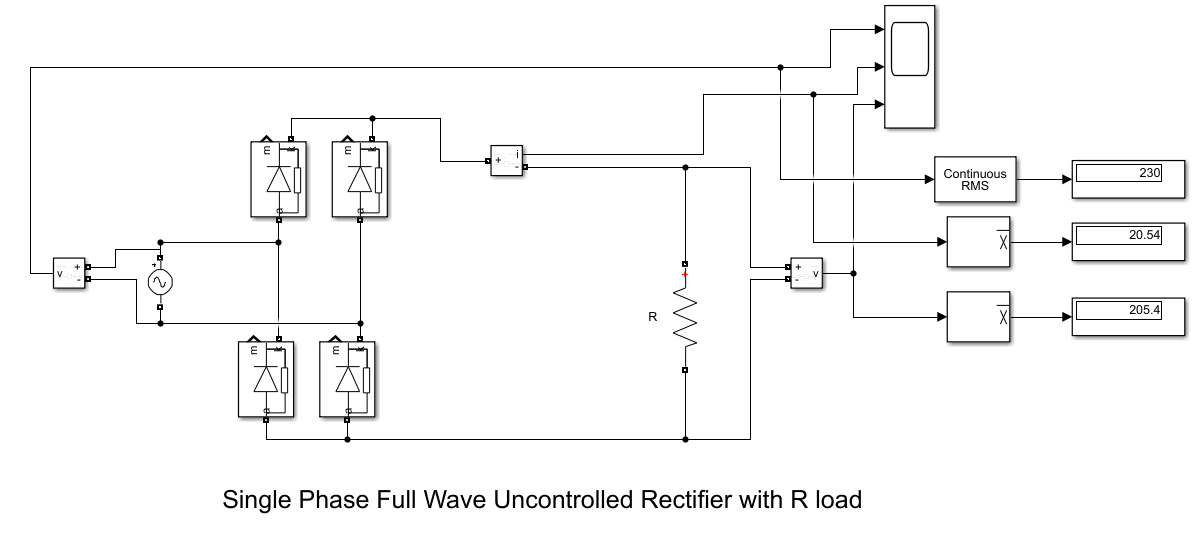
\includegraphics[width=0.7\textwidth]{images/experiment-2/circuit-diagram-simulation-01.png}
    \caption{Circuit used for simulation}
    \label{Fig_simulation_circuit_single-phase-full-wave-uncontrolled-rectifier-with-R-load}
\end{figure}

\subsection{Components Required}

\begin{table}[h]
    \renewcommand{\arraystretch}{1.3}
    \label{table_components_required_circuit_1}
    \centering
    \begin{tabular}{|c|c|c|c|}
        \hline
        Sr. No & Parameters                     & Ratings            & Quantity \\
        \hline
        \hline
        1      & AC Single Phase Voltage Source & 230V ($ V_{rms} $) & 1        \\
        \hline
        2      & Resistor                       & 10$ \Omega $       & 1        \\
        \hline
        3      & Diode                          & -                  & 1        \\
        \hline
        4      & Voltmeter                      & -                  & 2        \\
        \hline
        5      & Ammeter                        & -                  & 1        \\
        \hline
    \end{tabular}
    \caption{Components for Single Phase Full Wave Uncontrolled Rectifier with R load}

\end{table}




\subsection{Observations}

\begin{table}[h]
    \renewcommand{\arraystretch}{1.3}
    \label{table_observation_circuit_1}
    \centering
    \begin{tabular}{|c|c|c|}
        \hline
        Parameters                              & Theoretical Values & Simulation Values \\
        \hline
        \hline
        AC Input Voltage ($ V_{in,rms} $)       & 230V               & 230V              \\
        \hline
        Output Average Voltage ($ V_{o,avg} $)  & 207.07V            & 204.3V            \\
        \hline
        Output Average Current ($ I_{o,avg}  $) & 20.70A             & 20.43A            \\
        \hline
        DC Input Power ($ P_{DC}  $)            & 4218.916W          & 4173W             \\
        \hline
        Efficiency (\%)                         & 79.73              & 79.73             \\
        \hline
    \end{tabular}
    \caption{Observations for Single Phase Full Wave Uncontrolled Rectifier with R load}

\end{table}


Upon careful observation, it can be inferred that the simulated values exhibit a close resemblance to their theoretical counterparts. Given that the load is resistive, the output current waveform is found to be in phase with the output voltage waveform. Moreover, it is worth noting that as a result of full-wave rectification of the input AC signal, the output DC signal is characterized by a frequency that is double that of the input signal.
\pagebreak

\subsection{Resultant Waveforms}

% figure that is centered on the page
\begin{figure}[h]
    \centering
    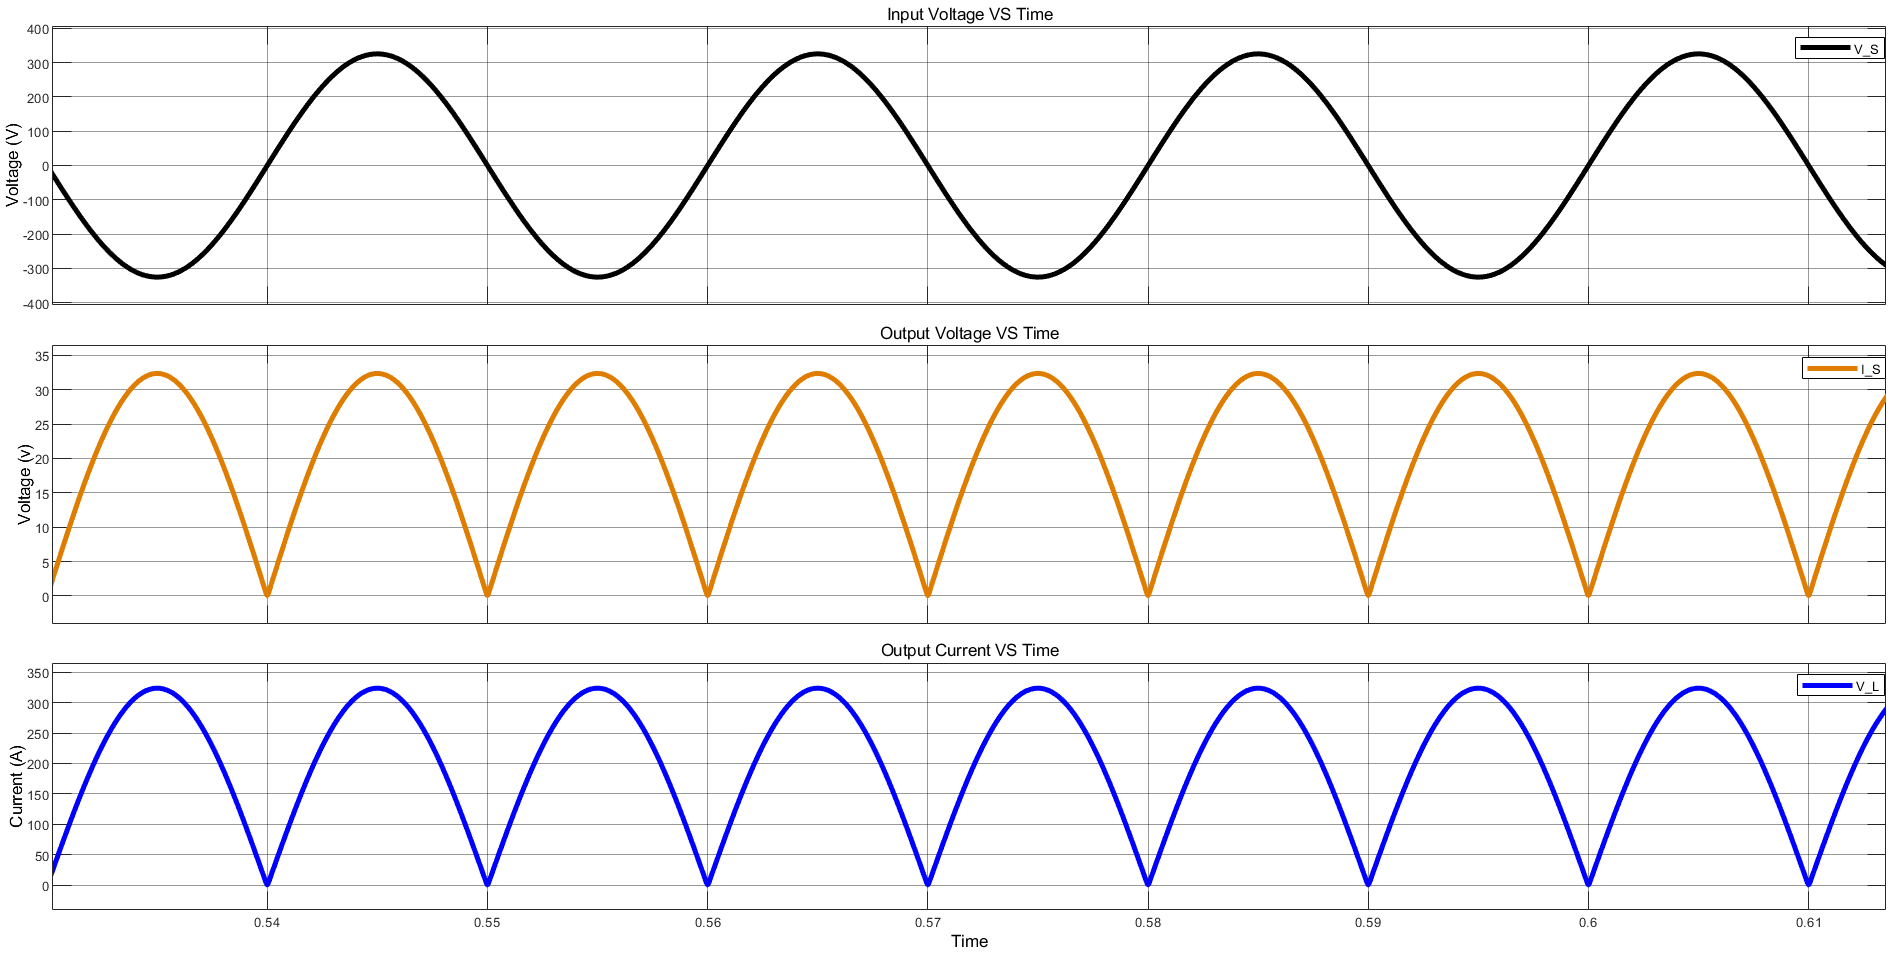
\includegraphics[width=1\textwidth]{images/experiment-2/circuit-scope-simulation-01.png}
    \caption{Scope Waveforms for Single Phase Full Wave Uncontrolled Rectifier with R load waveforms}
    \label{Fig_waveform_single-phase-full-wave-uncontrolled-rectifier-with-R-load}
\end{figure}

\pagebreak
\section{Single Phase Full Wave Controlled Rectifier with
  R load}

\subsection{Circuit used for simulation}

% figure that is centered on the page
\begin{figure}[h]
    \centering
    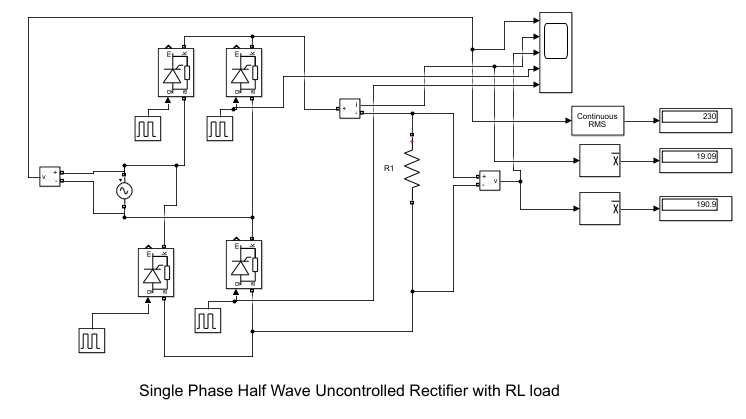
\includegraphics[width=0.7\textwidth]{images/experiment-2/circuit-diagram-simulation-02.png}
    \caption{Circuit used for simulation}
    \label{Fig_simulation_circuit_single-phase-full-wave-controlled-rectifier-with-R-load}
\end{figure}

\subsection{Components Required}

\begin{table}[h]
    \renewcommand{\arraystretch}{1.3}
    \label{table_components_required_circuit_2}
    \centering
    \begin{tabular}{|c|c|c|c|}
        \hline
        Sr. No & Parameters                     & Ratings            & Quantity \\
        \hline
        \hline
        1      & AC Single Phase Voltage Source & 230V ($ V_{rms} $) & 1        \\
        \hline
        2      & Resistor                       & 10$ \Omega $       & 1        \\
        \hline
        3      & Inductor                       & 10mH               & 1        \\
        \hline
        4      & Diode                          & -                  & 1        \\
        \hline
        5      & Voltmeter                      & -                  & 2        \\
        \hline
        6      & Ammeter                        & -                  & 1        \\
        \hline
    \end{tabular}
    \caption{Components for Single Phase Half Wave Uncontrolled Rectifier with RL load}
\end{table}


\subsection{Observations}

\begin{table}[h]
    \renewcommand{\arraystretch}{1.3}
    \label{table_observation_2}
    \centering
    \begin{tabular}{|c|c|c|}
        \hline
        Parameters                              & Theoretical Values & Simulation Values \\
        \hline
        \hline
        AC Input Voltage ($ V_{in,rms} $)       & 230V               & 230V              \\
        \hline
        Output Average Voltage ($ V_{o,avg} $)  & 193.2V             & 190.9V            \\
        \hline
        Output Average Current ($ I_{o,avg}  $) & 19.32A             & 19.09A            \\
        \hline
        AC Input Power ($ P_{AC} $)             & 2389.5 (W)         & 2318 (W)          \\
        \hline
        DC Input Power ($ P_{DC} $)             & 1071.53 (W)        & 1017 (W)          \\
        \hline
        Efficiency (\%)                         & 44.84              & 43.84             \\
        \hline
    \end{tabular}
    \caption{Observations for Single Phase Half Wave Uncontrolled Rectifier with RL load}

\end{table}


The circuit is designed to operate as a full bridge uncontrolled rectifier, but it will not produce any output voltage until firing pulses are applied to the thyristor gates. Once the thyristors are triggered, the circuit simulates a full bridge uncontrolled rectifier. The simulated values match the theoretical values closely. Because the load in the circuit is resistive, the output current is in phase with the output voltage. The output DC signal has a frequency that is twice that of the input AC signal.
The efficiency of uncontrolled rectifier with RL load is 44.84\%.
\pagebreak


\subsection{Resultant Waveforms}

% figure that is centered on the page
\begin{figure}[h]
    \centering
    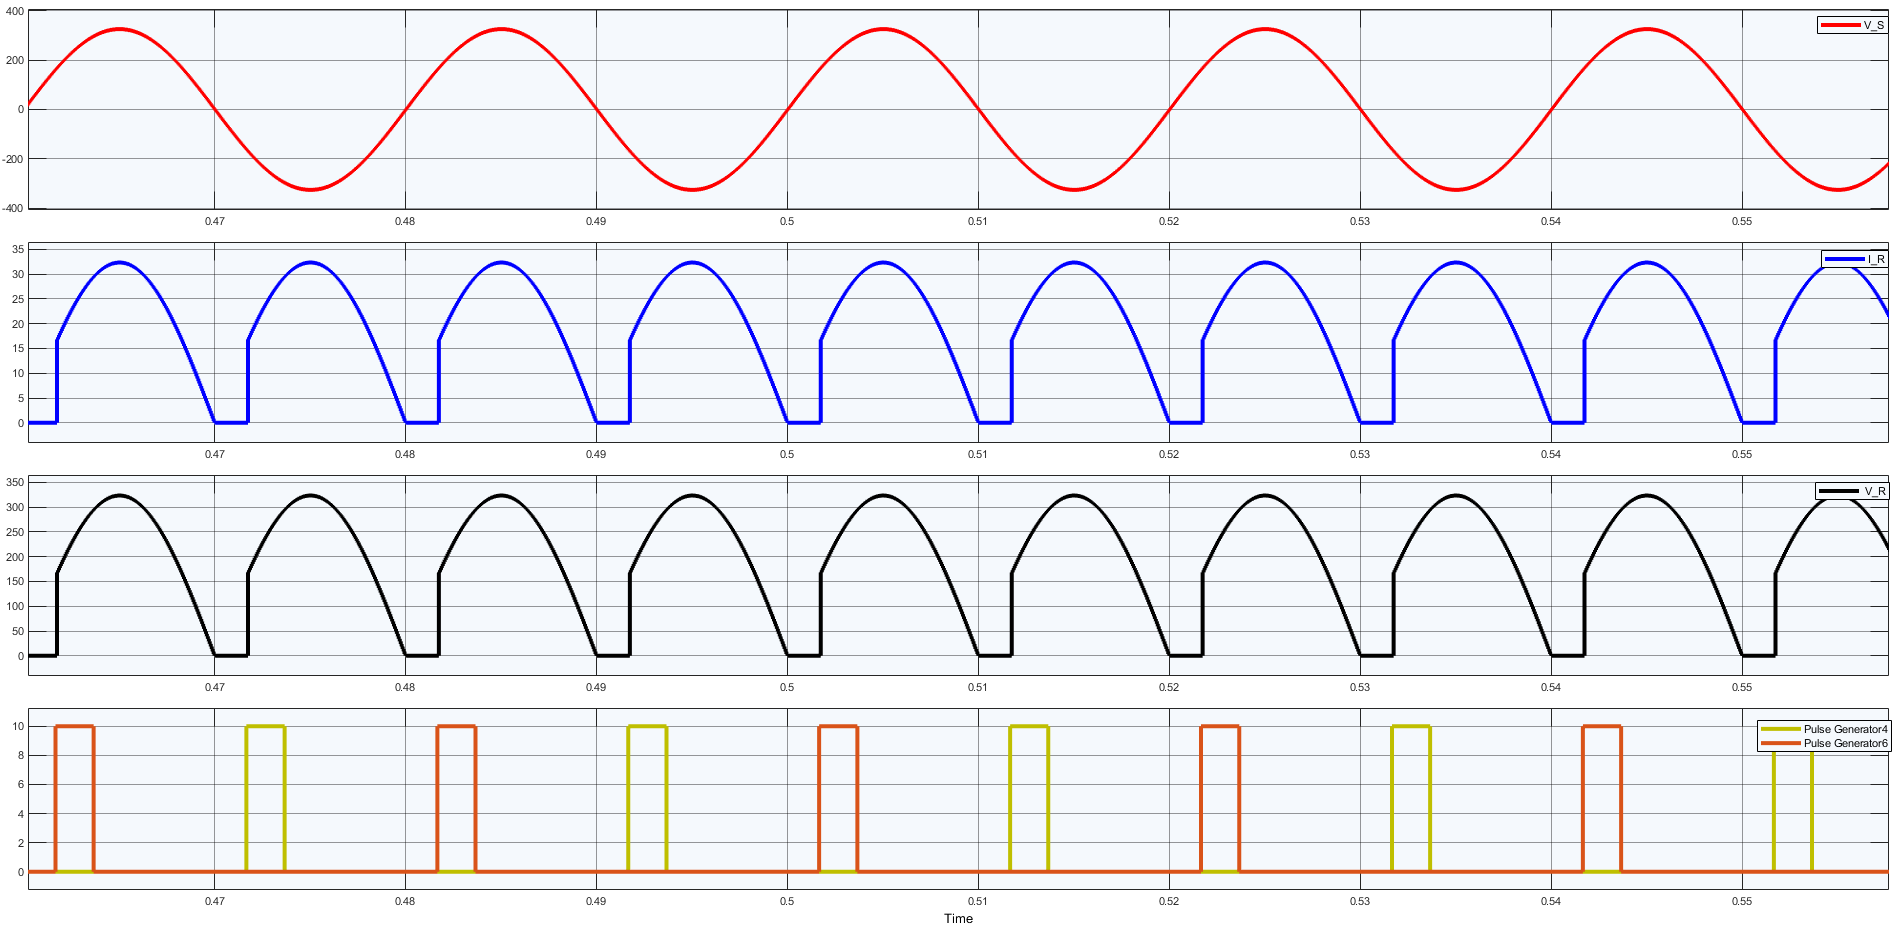
\includegraphics[width=1\textwidth]{images/experiment-2/circuit-scope-simulation-02.png}
    \caption{Scope Waveforms for Single Phase Half Wave Uncontrolled Rectifier with RL load}
    \label{Fig_waveform_single-phase-full-wave-controlled-rectifier-with-R-load}
\end{figure}

\pagebreak

\section{Single Phase Full Wave Controlled Rectifier with RL load}

\subsection{Circuit used for simulation}

% figure that is centered on the page
\begin{figure}[h]
    \centering
    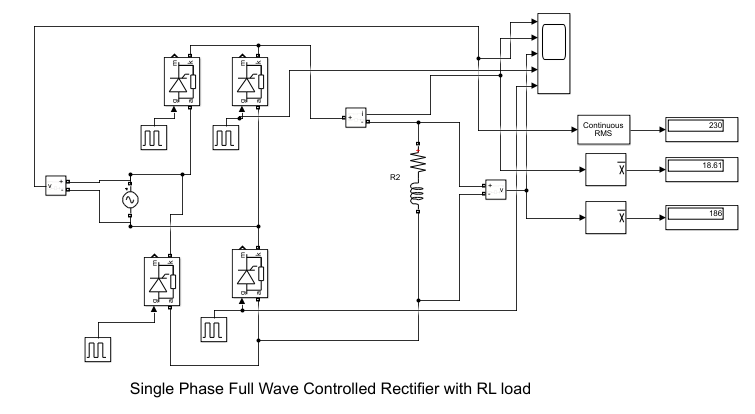
\includegraphics[width=0.7\textwidth]{images/experiment-2/circuit-diagram-simulation-03.png}
    \caption{Circuit used for simulation}
    \label{Fig_simulation_circuit_single-phase-full-wave-controlled-rectifier-with-RL-load}
\end{figure}

\subsection{Components Required}

\begin{table}[h]
    \renewcommand{\arraystretch}{1.3}
    \label{table_components_required_circuit_3}
    \centering
    \begin{tabular}{|c|c|c|c|}
        \hline
        Sr. No & Parameters                     & Ratings            & Quantity \\
        \hline
        \hline
        1      & AC Single Phase Voltage Source & 230V ($ V_{rms} $) & 1        \\
        \hline
        2      & Resistor                       & 10$ \Omega $       & 1        \\
        \hline
        3      & Inductor                       & 10mH               & 1        \\
        \hline
        4      & Diode                          & -                  & 1        \\
        \hline
        5      & Voltmeter                      & -                  & 2        \\
        \hline
        6      & Ammeter                        & -                  & 1        \\
        \hline
    \end{tabular}
    \caption{Components for Single Phase Half Wave Uncontrolled Rectifier with RL load and Freewheeling Diode}
\end{table}


\subsection{Observations}

\begin{table}[h]
    \renewcommand{\arraystretch}{1.3}
    \label{table_observation_3}
    \centering
    \begin{tabular}{|c|c|c|}
        \hline
        Parameters                              & Theoretical Values & Simulation Values \\
        \hline
        \hline
        AC Input Voltage ($ V_{in,rms} $)       & 230V               & 230V              \\
        \hline
        Output Average Voltage ($ V_{o,avg} $)  & 103.53V            & 103V              \\
        \hline
        Output Average Current ($ I_{o,avg}  $) & 10.35A             & 10.3A             \\
        \hline
        AC Input Power ($ P_{AC}  $)            & 2389.5 (W)         & 2266 (W)          \\
        \hline
        DC Input Power ($ P_{DC}  $)            & 1071.53 (W)        & 1015 (W)          \\
        \hline
        Efficiency (\%)                         & 44.84              & 44.8              \\
        \hline
    \end{tabular}
    \caption{Observations for Single Phase Half Wave Uncontrolled Rectifier with RL load and Freewheeling Diode}

\end{table}



Theoretical values are matched precisely by the simulated values. The full bridge rectifier with RL load produces output similar to the half-bridge rectifier with RL load when gate pulses are applied, except with double the frequency. The output current lags behind the output voltage due to the load's inductive nature, causing the thyristors to turn off later. This creates a momentary negative output voltage as the thyristors in the rectifier legs briefly allow for the negative half cycle of the AC voltage signal to conduct.
The efficiency of uncontrolled rectifier with RL load with freewheeling diode is 44.8\%.

\pagebreak

\subsection{Resultant Waveforms}


% figure that is centered on the page
\begin{figure}[h]
    \centering
    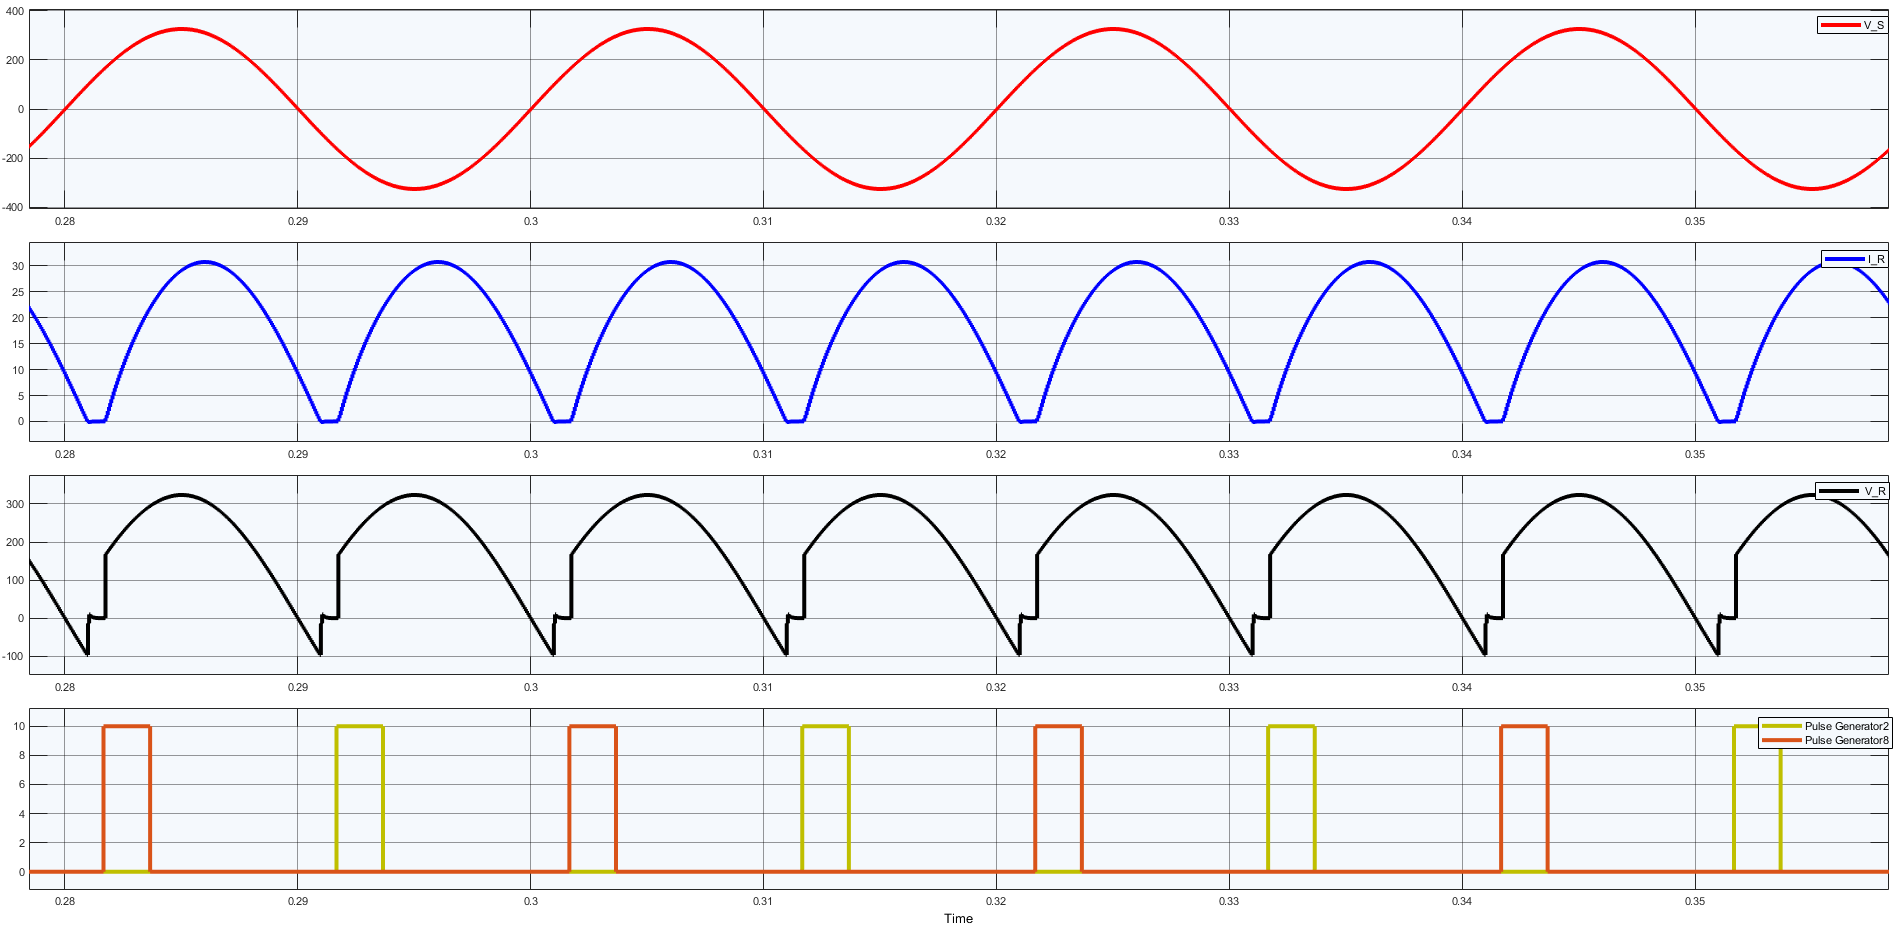
\includegraphics[width=1\textwidth]{images/experiment-2/circuit-scope-simulation-03.png}
    \caption{Scope Waveforms for Single Phase Half Wave Uncontrolled Rectifier with RL load and Freewheeling Diode}
    \label{Fig_waveform_single-phase-full-wave-controlled-rectifier-with-RL-load}
\end{figure}


\pagebreak



\section{Conclusion}


\hspace{\parindent}

Utilizing the MATLAB Simulink platform, the design of single phase full wave rectifiers with both controlled and uncontrolled R and RL loads was carried out with remarkable success. Voltage and current output waveforms were attained and output parameter values, both theoretically calculated and simulated, were juxtaposed.
The full-wave uncontrolled rectifier's efficiencies with R and RL load are measured to be 89.32\%. Furthermore, the full-wave controlled rectifier's efficiencies with R and RL load were measured to be 83.41\% and 81.33\%, respectively.

In conclusion, the full-wave rectifier is a more efficient and practical alternative to the half-wave rectifier because it produces a smoother DC output, has a higher output voltage and lower output ripple. The four diodes used in a bridge configuration ensure that the input AC voltage is rectified, producing a DC output voltage across the output terminals.
This process of rectification produces a unidirectional DC output signal that can be used for various applications.
The average output voltage and current for full-wave rectifiers with R load can be calculated using the above equations. It is important to note that these calculations are based on idealized conditions and practical circuits may have additional factors that affect their performance.
\pagebreak